\documentclass[english, twocolumn, 10pt, aps, superscriptaddress, floatfix, prb, citeautoscript]{revtex4-1}
\pdfoutput=1
\usepackage[utf8]{inputenc}
\usepackage[T1]{fontenc}
\usepackage{verbatim}
\usepackage{units}
\usepackage{mathtools}
\usepackage{amsmath}
\usepackage{amssymb}
\usepackage{graphicx}
\usepackage{wasysym}
\usepackage{layouts}
\usepackage{siunitx}
\usepackage{bm}
\usepackage{xcolor}
\usepackage[colorlinks, citecolor={blue!50!black}, urlcolor={blue!50!black}, linkcolor={red!50!black}]{hyperref}
\usepackage{bookmark}
\usepackage{tabularx}
\usepackage{microtype}
\usepackage{babel}
\hypersetup{pdfauthor={Bas Nijholt, Anton Akhmerov},pdftitle={Great and
certainly not overstated contribution to the literature}}

\setcounter{secnumdepth}{4}
\setcounter{tocdepth}{4}

\DeclareMathOperator{\e}{e}
\DeclareMathOperator{\de}{d\!}
\DeclareMathOperator{\Tr}{Tr}
\DeclareMathOperator{\diag}{diag}
\DeclareMathOperator{\Res}{Res}
\DeclareMathOperator{\sgn}{sgn}
\DeclareMathOperator{\Pf}{Pf}
\DeclareMathOperator{\Det}{Det}
\DeclareMathOperator{\rank}{rank}
\DeclareMathOperator{\im}{Im}
\DeclareMathOperator{\re}{Re}
\newcommand{\kx}{k_x}
\newcommand{\ky}{k_y}
\newcommand{\meff}{m_\text{eff}}

\renewcommand{\comment}[2]{#2}
% Uncomment the following line for paragraph descriptions to appear in the file.
\renewcommand{\comment}{\paragraph}

\DeclarePairedDelimiter\abs{\lvert}{\rvert}
\DeclarePairedDelimiter\norm{\lVert}{\rVert}

\makeatletter
\let\oldabs\abs
\def\abs{\@ifstar{\oldabs}{\oldabs*}}
\let\oldnorm\norm
\def\norm{\@ifstar{\oldnorm}{\oldnorm*}}
\makeatother

\newcommand{\ev}[1]{\langle#1\rangle}
\newcommand{\bra}[1]{\langle#1|}
\newcommand{\ket}[1]{|#1\rangle}
\newcommand{\bracket}[2]{\langle#1|#2\rangle}

\newcolumntype{L}[1]{>{\raggedright\arraybackslash}p{#1}}
\newcolumntype{C}[1]{>{\centering\arraybackslash}p{#1}}
\newcolumntype{R}[1]{>{\raggedleft\arraybackslash}p{#1}}

% workaround for https://github.com/jgm/pandoc/issues/2392#issuecomment-140114736
\renewcommand{\citep}{\cite}

\begin{document}

\title{Great and certainly not overstated contribution to the
literature}

\author{Bas Nijholt}
\email[Electronic address: ]{bas@nijho.lt}
\affiliation{TU Delft}
\affiliation{Station Q}
\author{Anton Akhmerov}
\email[Electronic address: ]{i@antonakhmerov.org}
\affiliation{TU Delft}

\date{\today}

\begin{abstract}
Lorem ipsum dolor sit amet, consectetur adipiscing elit, sed do eiusmod
tempor incididunt ut labore et dolore magna aliqua. Ut enim ad minim
veniam, quis nostrud exercitation ullamco laboris nisi ut aliquip ex ea
commodo consequat. Duis aute irure dolor in reprehenderit in voluptate
velit esse cillum dolore eu fugiat nulla pariatur. Excepteur sint
occaecat cupidatat non proident, sunt in culpa qui officia deserunt
mollit anim id est laborum.
\end{abstract}

\flushbottom
\maketitle

\hypertarget{introduction}{%
\section{Introduction}\label{introduction}}

Lorem ipsum dolor sit amet, consectetur adipiscing elit, sed do eiusmod
tempor incididunt ut labore et dolore magna aliqua. Ut enim ad minim
veniam, quis nostrud exercitation ullamco laboris nisi ut aliquip ex ea
commodo consequat. Duis aute irure dolor in reprehenderit in voluptate
velit esse cillum dolore eu fugiat nulla pariatur. Excepteur sint
occaecat cupidatat non proident, sunt in culpa qui officia deserunt
\textbf{mollit anim id est} laborum.

References are cited as \citep{nijholt2016orbital}.

\hypertarget{methods}{%
\section{Methods}\label{methods}}

Footnotes can be entered using this code\footnote{a footnote}.

Figures are included like this.

\begin{figure}
\hypertarget{fig:dummy}{%
\centering
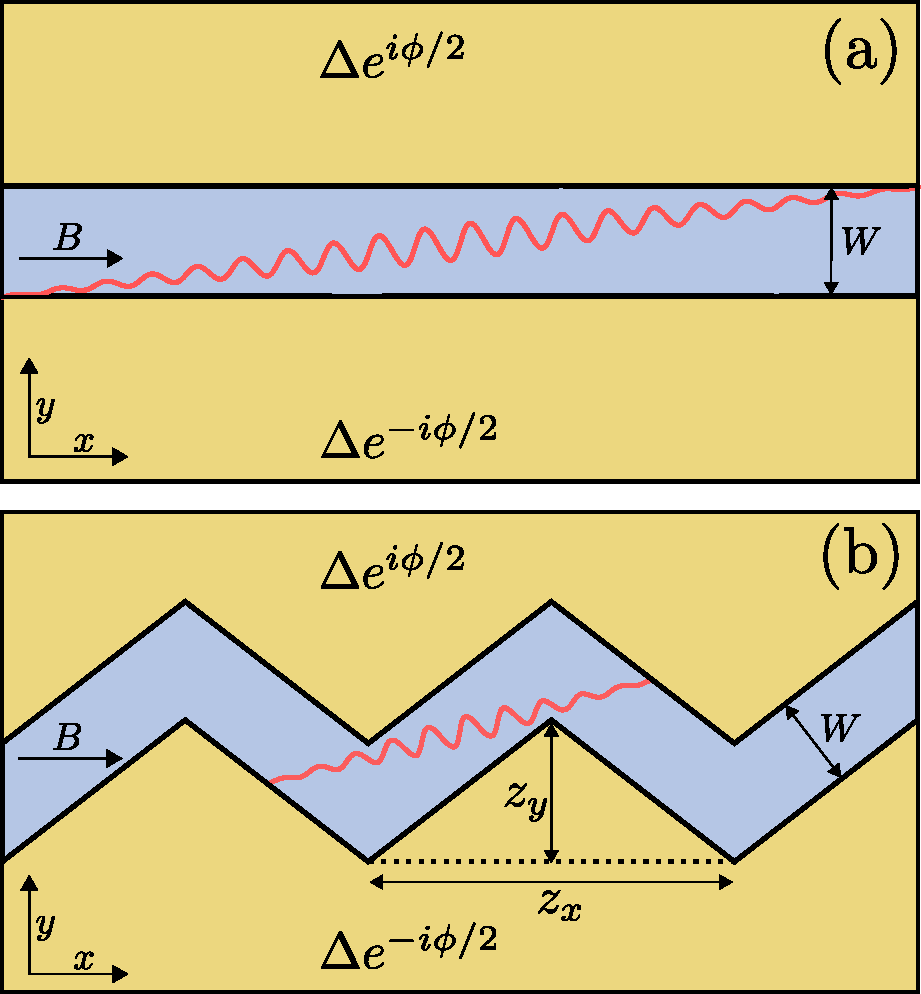
\includegraphics{figures/dummy.pdf}
\caption{This is gonna be the caption.}\label{fig:dummy}
}
\end{figure}

And referenced from here as Fig. \ref{fig:dummy}.

Complex tables can use standard LaTeX code as this one.

Equations can be used inline \(y=\beta_0 + \beta_1 x + \epsilon\) or as
usual
\begin{equation}\protect\hypertarget{eq:example_eq}{}{f(x)=\frac{1}{x}}\label{eq:example_eq}\end{equation}
and referenced with Eq. \eqref{eq:example_eq}.

\begin{table}[ht]
  \begin{center}
    \caption{Your first table.}
    \label{tab:table1}
    \begin{tabular}{l|c|r}
      \textbf{Value 1} & \textbf{Value 2} & \textbf{Value 3}\\
      $\alpha$ & $\beta$ & $\gamma$ \\
      \hline
      1 & 1110.1 & a\\
      2 & 10.1 & b\\
      3 & 23.113231 & c\\
    \end{tabular}
  \end{center}
\end{table}

\hypertarget{results}{%
\section{Results}\label{results}}

\hypertarget{discussion}{%
\section{Discussion}\label{discussion}}

\section*{Acknowledgements}
We'd like to thank \ldots{}

\section*{Author contributions statement}
B.N. created the template with input from J.W. A.A. is a place holder.
All authors looked at the manuscript.


\bibliographystyle{apsrev4-1}
\bibliography{paper.bib}

\end{document}
